%% uncomment to list all files in log
%\listfiles

\documentclass[12pt]{report}


\usepackage{fontspec}

%\setmainfont[Scale=MatchLowercase]{Lucida Bright}
%\setmonofont{FreeMono}
%\setmonofont{Source Code Pro}
\setmonofont[Scale=MatchLowercase]{Ubuntu Mono}

\usepackage[headings]{fullpage}

% national use characters 
%\usepackage{inputenc}

% ams mathematical symbols
\usepackage{amsmath,amssymb}

% added to support pandoc highlighting
\usepackage{microtype}

\usepackage{makeidx}

% add index and bibliographies to table of contents
\usepackage[nottoc]{tocbibind}

% postscript courier and times in place of cm fonts
%\usepackage{courier}
%\usepackage{times}

% extended coloring
\usepackage{color}
\usepackage[table,dvipsnames]{xcolor}
\usepackage{colortbl}

% advanced date formating
\usepackage{datetime}

%support pandoc code highlighting
\usepackage{fancyvrb}
\DefineShortVerb[commandchars=\\\{\}]{\|}
\DefineVerbatimEnvironment{Highlighting}{Verbatim}{commandchars=\\\{\}}
% Add ',fontsize=\small' for more characters per line

%tango style colors
% \usepackage{framed}
% \definecolor{shadecolor}{RGB}{255,255,255}
% \newenvironment{Shaded}{\begin{snugshade}}{\end{snugshade}}
% \newcommand{\KeywordTok}[1]{\textcolor[rgb]{0.13,0.29,0.53}{\textbf{{#1}}}}
% \newcommand{\DataTypeTok}[1]{\textcolor[rgb]{0.13,0.29,0.53}{{#1}}}
% \newcommand{\DecValTok}[1]{\textcolor[rgb]{0.00,0.00,0.81}{{#1}}}
% \newcommand{\BaseNTok}[1]{\textcolor[rgb]{0.00,0.00,0.81}{{#1}}}
% \newcommand{\FloatTok}[1]{\textcolor[rgb]{0.00,0.00,0.81}{{#1}}}
% \newcommand{\CharTok}[1]{\textcolor[rgb]{0.31,0.60,0.02}{{#1}}}
% \newcommand{\StringTok}[1]{\textcolor[rgb]{0.31,0.60,0.02}{{#1}}}
% \newcommand{\CommentTok}[1]{\textcolor[rgb]{0.56,0.35,0.01}{\textit{{#1}}}}
% \newcommand{\OtherTok}[1]{\textcolor[rgb]{0.56,0.35,0.01}{{#1}}}
% \newcommand{\AlertTok}[1]{\textcolor[rgb]{0.94,0.16,0.16}{{#1}}}
% \newcommand{\FunctionTok}[1]{\textcolor[rgb]{0.00,0.00,0.00}{{#1}}}
% \newcommand{\RegionMarkerTok}[1]{{#1}}
% \newcommand{\ErrorTok}[1]{\textbf{{#1}}}
% \newcommand{\NormalTok}[1]{{#1}}

%espresso style colors
% \usepackage{framed}
% \definecolor{shadecolor}{RGB}{42,33,28}
% \newenvironment{Shaded}{\begin{snugshade}}{\end{snugshade}}
% \newcommand{\KeywordTok}[1]{\textcolor[rgb]{0.26,0.66,0.93}{\textbf{{#1}}}}
% \newcommand{\DataTypeTok}[1]{\textcolor[rgb]{0.74,0.68,0.62}{\underline{{#1}}}}
% \newcommand{\DecValTok}[1]{\textcolor[rgb]{0.27,0.67,0.26}{{#1}}}
% \newcommand{\BaseNTok}[1]{\textcolor[rgb]{0.27,0.67,0.26}{{#1}}}
% \newcommand{\FloatTok}[1]{\textcolor[rgb]{0.27,0.67,0.26}{{#1}}}
% \newcommand{\CharTok}[1]{\textcolor[rgb]{0.02,0.61,0.04}{{#1}}}
% \newcommand{\StringTok}[1]{\textcolor[rgb]{0.02,0.61,0.04}{{#1}}}
% \newcommand{\CommentTok}[1]{\textcolor[rgb]{0.00,0.40,1.00}{\textit{{#1}}}}
% \newcommand{\OtherTok}[1]{\textcolor[rgb]{0.74,0.68,0.62}{{#1}}}
% \newcommand{\AlertTok}[1]{\textcolor[rgb]{1.00,1.00,0.00}{{#1}}}
% \newcommand{\FunctionTok}[1]{\textcolor[rgb]{1.00,0.58,0.35}{\textbf{{#1}}}}
% \newcommand{\RegionMarkerTok}[1]{\textcolor[rgb]{0.74,0.68,0.62}{{#1}}}
% \newcommand{\ErrorTok}[1]{\textcolor[rgb]{0.74,0.68,0.62}{\textbf{{#1}}}}
% \newcommand{\NormalTok}[1]{\textcolor[rgb]{0.74,0.68,0.62}{{#1}}}

%kete style colors
% \newenvironment{Shaded}{}{}
% \newcommand{\KeywordTok}[1]{\textbf{{#1}}}
% \newcommand{\DataTypeTok}[1]{\textcolor[rgb]{0.50,0.00,0.00}{{#1}}}
% \newcommand{\DecValTok}[1]{\textcolor[rgb]{0.00,0.00,1.00}{{#1}}}
% \newcommand{\BaseNTok}[1]{\textcolor[rgb]{0.00,0.00,1.00}{{#1}}}
% \newcommand{\FloatTok}[1]{\textcolor[rgb]{0.50,0.00,0.50}{{#1}}}
% \newcommand{\CharTok}[1]{\textcolor[rgb]{1.00,0.00,1.00}{{#1}}}
% \newcommand{\StringTok}[1]{\textcolor[rgb]{0.87,0.00,0.00}{{#1}}}
% \newcommand{\CommentTok}[1]{\textcolor[rgb]{0.50,0.50,0.50}{\textit{{#1}}}}
% \newcommand{\OtherTok}[1]{{#1}}
% \newcommand{\AlertTok}[1]{\textcolor[rgb]{0.00,1.00,0.00}{\textbf{{#1}}}}
% \newcommand{\FunctionTok}[1]{\textcolor[rgb]{0.00,0.00,0.50}{{#1}}}
% \newcommand{\RegionMarkerTok}[1]{{#1}}
% \newcommand{\ErrorTok}[1]{\textcolor[rgb]{1.00,0.00,0.00}{\textbf{{#1}}}}
% \newcommand{\NormalTok}[1]{{#1}}
%end pandoc code hacks

% jodliterate colors
\usepackage{color}
\definecolor{shadecolor}{RGB}{248,248,248}
% j control structures 
\definecolor{keywcolor}{rgb}{0.13,0.29,0.53}
% j explicit arguments x y m n u v
\definecolor{datacolor}{rgb}{0.13,0.29,0.53}
% j numbers - all types see j.xml
\definecolor{decvcolor}{rgb}{0.00,0.00,0.81}
\definecolor{basencolor}{rgb}{0.00,0.00,0.81}
\definecolor{floatcolor}{rgb}{0.00,0.00,0.81}
% j local assignments
\definecolor{charcolor}{rgb}{0.31,0.60,0.02}
\definecolor{stringcolor}{rgb}{0.31,0.60,0.02}
\definecolor{commentcolor}{rgb}{0.56,0.35,0.01}
% primitive adverbs and conjunctions
%\definecolor{othercolor}{rgb}{0.56,0.35,0.01}   
\definecolor{othercolor}{RGB}{0,0,255}
% global assignments
\definecolor{alertcolor}{rgb}{0.94,0.16,0.16}
% primitive J verbs and noun names
\definecolor{funccolor}{rgb}{0.00,0.00,0.00}    

\usepackage{framed}
\newenvironment{Shaded}{}{}
\newcommand{\KeywordTok}[1]{\textcolor{keywcolor}{\textbf{{#1}}}}
\newcommand{\DataTypeTok}[1]{\textcolor{datacolor}{{#1}}}
%\newcommand{\DecValTok}[1]{\textcolor{decvcolor}{{#1}}}
\newcommand{\DecValTok}[1]{{#1}} 
\newcommand{\BaseNTok}[1]{\textcolor{basencolor}{{#1}}}
\newcommand{\FloatTok}[1]{\textcolor{floatcolor}{{#1}}}
\newcommand{\CharTok}[1]{\textcolor{charcolor}{\textbf{{#1}}}}
\newcommand{\StringTok}[1]{\textcolor{stringcolor}{{#1}}}
\newcommand{\CommentTok}[1]{\textcolor{commentcolor}{\textit{{#1}}}}
\newcommand{\OtherTok}[1]{\textcolor{othercolor}{{#1}}} 
\newcommand{\AlertTok}[1]{\textcolor{alertcolor}{\textbf{{#1}}}}
%\newcommand{\FunctionTok}[1]{\textcolor{funccolor}{{#1}}}
\newcommand{\FunctionTok}[1]{{#1}}
\newcommand{\RegionMarkerTok}[1]{{#1}}
\newcommand{\ErrorTok}[1]{\textbf{{#1}}}
\newcommand{\NormalTok}[1]{{#1}}

% headers and footers
\usepackage{fancyhdr}
\pagestyle{fancy}

\fancyhead{}
\fancyfoot{}

%\fancyhead[LE,RO]{\slshape \rightmark}
%\fancyhead[LO,RE]{\slshape \leftmark}
\fancyfoot[C]{\thepage}
%\headrulewidth 0.4pt
%\footrulewidth 0 pt

%\addtolength{\headheight}{\baselineskip}

%\lfoot{\emph{Analyze the Data not the Drivel}}
%\rfoot{\emph{\today}}

% subfigure handles figures that contain subfigures
%\usepackage{color,graphicx,subfigure,sidecap}
\usepackage{graphicx,sidecap}
\usepackage{subfigure}
\graphicspath{{./inclusions/}}

% floatflt provides for text wrapping around small figures and tables
\usepackage{floatflt}

% tweak caption formats 
\usepackage{caption} 
\usepackage{sidecap}
%\usepackage{subcaption} % not compatible with subfigure

\usepackage{rotating} % flip tables sideways

% complex footnotes
%\usepackage{bigfoot}

% weird logos \XeLaTeX
\usepackage{metalogo}

% source code listings
\usepackage{listings}

% long tables
% \usepackage{longtable}

\newcommand{\HRule}{\rule{\linewidth}{0.5mm}}

% map LaTeX cross references into PDF cross references
\usepackage[
            %dvips,
            colorlinks,
            linkcolor=blue,
            citecolor=blue,
            urlcolor=blue,   % magenta, cyan default        
            pdfauthor={John D. Baker},
            pdftitle={Analyze the Data not the Drivel},
            pdfsubject={Blog},
            pdfcreator={MikTeX+LaTeXe with hyperref package},
            pdfkeywords={blog,wordpress},
            ]{hyperref}
           
% custom colors
\definecolor{CodeBackGround}{cmyk}{0.0,0.0,0,0.05}    % light gray
\definecolor{CodeComment}{rgb}{0,0.50,0.00}           % dark green {0,0.45,0.08}
\definecolor{TableStripes}{gray}{0.9}                 % odd/even background in tables

\lstdefinelanguage{bat}
{morekeywords={echo,title,pushd,popd,setlocal,endlocal,off,if,not,exist,set,goto,pause},
sensitive=True,
morecomment=[l]{rem}
}

\lstdefinelanguage{jdoc}
{
morekeywords={},
otherkeywords={assert.,break.,continue.,for.,do.,if.,else.,elseif.,return.,select.,end.
,while.,whilst.,throw.,catch.,catchd.,catcht.,try.,case.,fcase.},
sensitive=True,
morecomment=[l]{NB.},
morestring=[b]',
morestring=[d]',
}

% latex size ordering - can never remember it
% \tiny
% \scriptsize
% \footnotesize
% \small
% \normalsize
% \large
% \Large
% \LARGE
% \huge
% \Huge
 
% listings package settings  
\lstset{%
  language=jdoc,                                % j document settings
  basicstyle=\ttfamily\footnotesize,            
  keywordstyle=\bfseries\color{keywcolor}\footnotesize,
  identifierstyle=\color{black},
  commentstyle=\slshape\color{CodeComment},     % colored slanted comments
  stringstyle=\color{red}\ttfamily,
  showstringspaces=false,                       
  %backgroundcolor=\color{CodeBackGround},       
  frame=single,                                
  framesep=1pt,                                 
  framerule=0.8pt,                             
  rulecolor=\color{CodeBackGround},   
  showspaces=false,
  %columns=fullflexible,
  %numbers=left,
  %numberstyle=\footnotesize,
  %numbersep=9pt,
  tabsize=2,
  showtabs=false,
  captionpos=b
  breaklines=true,                              
  breakindent=5pt                              
}

\lstdefinelanguage{JavaScript}{
  keywords={typeof, new, true, false, catch, function, return, null, catch, switch, var, if, in, while, do, else, case, break},
  ndkeywords={class, export, boolean, throw, implements, import, this},
  ndkeywordstyle=\color{darkgray}\bfseries,
  sensitive=false,
  comment=[l]{//},
  morecomment=[s]{/*}{*/},
  morestring=[b]',
  morestring=[b]"
}

% C# settings
\lstdefinestyle{sharpc}{
language=[Sharp]C,
basicstyle=\ttfamily\scriptsize, 
keywordstyle=\bfseries\color{keywcolor}\scriptsize,
framerule=0pt
}

% for source code listing longer than two use smaller font
\lstdefinestyle{smallersource}{
basicstyle=\ttfamily\scriptsize, 
keywordstyle=\bfseries\color{keywcolor}\scriptsize,
framerule=0pt
}

\lstdefinestyle{resetdefaults}{
language=jdoc,
basicstyle=\ttfamily\footnotesize,  
keywordstyle=\bfseries\color{keywcolor}\footnotesize,                                                               
framerule=0.8pt 
}

% APL UTF8 code points listed for lstlisting processing
\makeatletter
\lst@InputCatcodes
\def\lst@DefEC{%
 \lst@CCECUse \lst@ProcessLetter
  ^^80^^81^^82^^83^^84^^85^^86^^87^^88^^89^^8a^^8b^^8c^^8d^^8e^^8f%
  ^^90^^91^^92^^93^^94^^95^^96^^97^^98^^99^^9a^^9b^^9c^^9d^^9e^^9f%
  ^^a0^^a1^^a2^^a3^^a4^^a5^^a6^^a7^^a8^^a9^^aa^^ab^^ac^^ad^^ae^^af%
  ^^b0^^b1^^b2^^b3^^b4^^b5^^b6^^b7^^b8^^b9^^ba^^bb^^bc^^bd^^be^^bf%
  ^^c0^^c1^^c2^^c3^^c4^^c5^^c6^^c7^^c8^^c9^^ca^^cb^^cc^^cd^^ce^^cf%
  ^^d0^^d1^^d2^^d3^^d4^^d5^^d6^^d7^^d8^^d9^^da^^db^^dc^^dd^^de^^df%
  ^^e0^^e1^^e2^^e3^^e4^^e5^^e6^^e7^^e8^^e9^^ea^^eb^^ec^^ed^^ee^^ef%
  ^^f0^^f1^^f2^^f3^^f4^^f5^^f6^^f7^^f8^^f9^^fa^^fb^^fc^^fd^^fe^^ff%
  ^^^^20ac^^^^0153^^^^0152%
  ^^^^20a7^^^^2190^^^^2191^^^^2192^^^^2193^^^^2206^^^^2207^^^^220a%
  ^^^^2218^^^^2228^^^^2229^^^^222a^^^^2235^^^^223c^^^^2260^^^^2261%
  ^^^^2262^^^^2264^^^^2265^^^^2282^^^^2283^^^^2296^^^^22a2^^^^22a3%
  ^^^^22a4^^^^22a5^^^^22c4^^^^2308^^^^230a^^^^2336^^^^2337^^^^2339%
  ^^^^233b^^^^233d^^^^233f^^^^2340^^^^2342^^^^2347^^^^2348^^^^2349%
  ^^^^234b^^^^234e^^^^2350^^^^2352^^^^2355^^^^2357^^^^2359^^^^235d%
  ^^^^235e^^^^235f^^^^2361^^^^2362^^^^2363^^^^2364^^^^2365^^^^2368%
  ^^^^236a^^^^236b^^^^236c^^^^2371^^^^2372^^^^2373^^^^2374^^^^2375%
  ^^^^2377^^^^2378^^^^237a^^^^2395^^^^25af^^^^25ca^^^^25cb%  
  ^^00}
\lst@RestoreCatcodes
\makeatother

% custom lengths used within minipages
\newcommand{\minindent}{17pt}


\makeindex

\begin{document}

\subsection*{\href{http://analyzethedatanotthedrivel.org/2021/01/12/new-year-new-image-editors/}{New Year New Image Editors}}
\addcontentsline{toc}{subsection}{New Year New Image Editors}


\noindent\emph{Posted: 12 Jan 2021 23:28:42}
\vspace{6pt}

We all have our New Year's traditions. One of mine is trying out
\emph{new}\footnote{New to me!} image editors and
reevaluating older familiar editors that I've put aside. This year I
looked at three editors.

\begin{enumerate}
\def\labelenumi{\arabic{enumi}.}
\tightlist
\item
  \href{https://skylum.com/luminar/luminar-ai}{Luminar AI}
\item
  \href{https://www.dl-c.com/Downloads.html}{Picture Window Pro 8}
\item
  \href{https://www.gimp.org/}{GNU GIMP 2.10.22}
\end{enumerate}

\paragraph{Luminar AI}\label{luminar-ai}

Let's start with \href{https://skylum.com/luminar/luminar-ai}{Luminar AI}. 
Luminar AI makes the possibly true claim that it's the first
commercially available ``AI-Driven'' image editor. Whenever
\emph{salespeople} concatenate qualifying phrases set your
\href{https://duckduckgo.com/?q=spinal+tap+set+to+11\&t=brave\&iax=videos\&ia=videos\&iai=https\%3A\%2F\%2Fwww.youtube.com\%2Fwatch\%3Fv\%3DF7IZZXQ89Oc}{bullshit
detector to eleven} and proceed skeptically.

To start, the entire field of ``Machine Learning,'' and all its little
subdisciplines like ``AI image processing,'' are horribly misnamed.
\href{https://xkcd.com/}{XKCD} pointed this out in this pithy cartoon: see Figure~\ref{fig:7048X0} on page~\pageref{fig:7048X0}.

%\href{https://xkcd.com/1838/}{
\includegraphics{xkcd_machine_learning.png}}

%\captionsetup[figure]{labelformat=empty}
%\begin{figure}[htbp]
%\centering
%
\includegraphics[width=0.40\textwidth]{xkcd_machine_learning.png}
%\label{fig:7048X0}
%\end{figure}

%\captionsetup[figure]{labelformat=empty}
\captionsetup[figure]{labelformat=default}
 \begin{SCfigure}[50]
 \centering
 \href{https://xkcd.com/1838/}{
\includegraphics[width=0.40\textwidth]{xkcd_machine_learning.png}}
 \caption{\href{https://xkcd.com/1838/}{XKCD} is umimpressed with the misleading moniker ``Machine Learning.''
Computer nerds name things as badly as suburban housing developers. Bad
terminology leads to muddled thinking. As hyperbolic screeching lefties
repeat \emph{ad nauseam}, \href{https://www.facebook.com/PoliticalHype/videos/401536327743389/}{``Words Matter!.''}
}
 \label{fig:7048X0}
 \end{SCfigure}


I don't know what you should call the many relatively novel image
processing algorithms found in products like Luminar AI but calling them
``intelligent'' completely misses the mark.

\begin{quote}
\emph{Only conscious and self-aware entities can be considered intelligent.}
\end{quote}

Luminar AI is not self-aware --- thank the
\href{https://www.spaghettimonster.org/}{all squiggly FSM} for that ---
I wouldn't want it in my house if it was!

Lucky for Luminar AI the only thing I ask of image editors is, ``do they
help me edit images?'' In Luminar's case, the answer is a
\emph{resounding} yes!

I'm a Luminar AI newbie but I already appreciate how it's simplified
some tedious editing tasks like sky replacement. Consider my
\emph{boring light} shot of the Devil's Tower in Wyoming: see Figure~\ref{fig:7048X1} on page~\pageref{fig:7048X1}.

%\href{https://conceptcontrol.smugmug.com/Trips/USA-and-Canada/Western-Road-Trip-2015/i-Dq2KDP4/A}{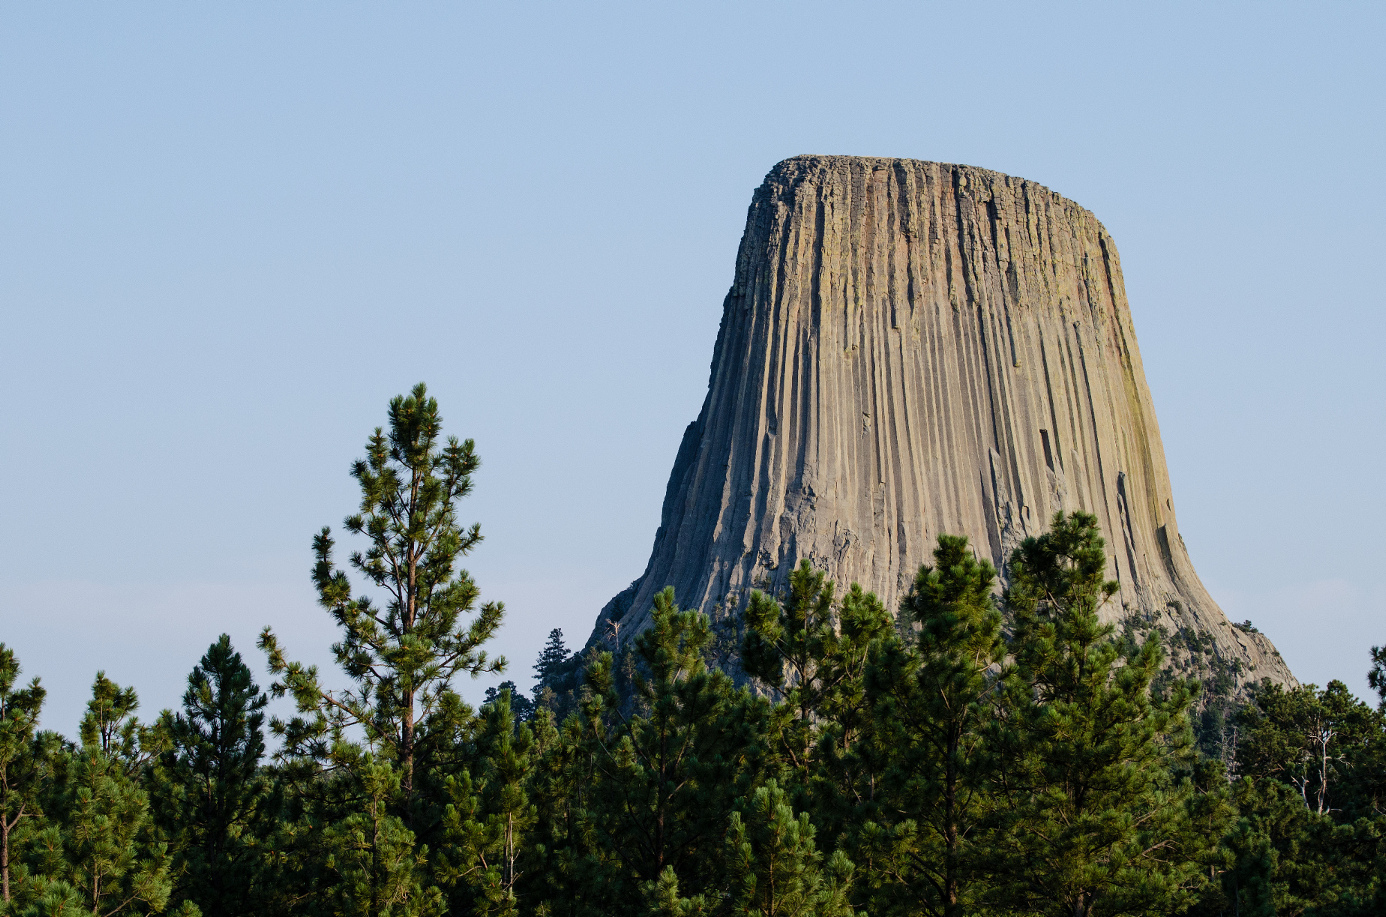
\includegraphics{devils_tower_bed_breakfast.jpg}}

%\captionsetup[figure]{labelformat=empty}
\captionsetup[figure]{labelformat=default}
\begin{figure}[htbp]
\centering
\href{https://conceptcontrol.smugmug.com/Trips/USA-and-Canada/Western-Road-Trip-2015/i-Dq2KDP4/A}{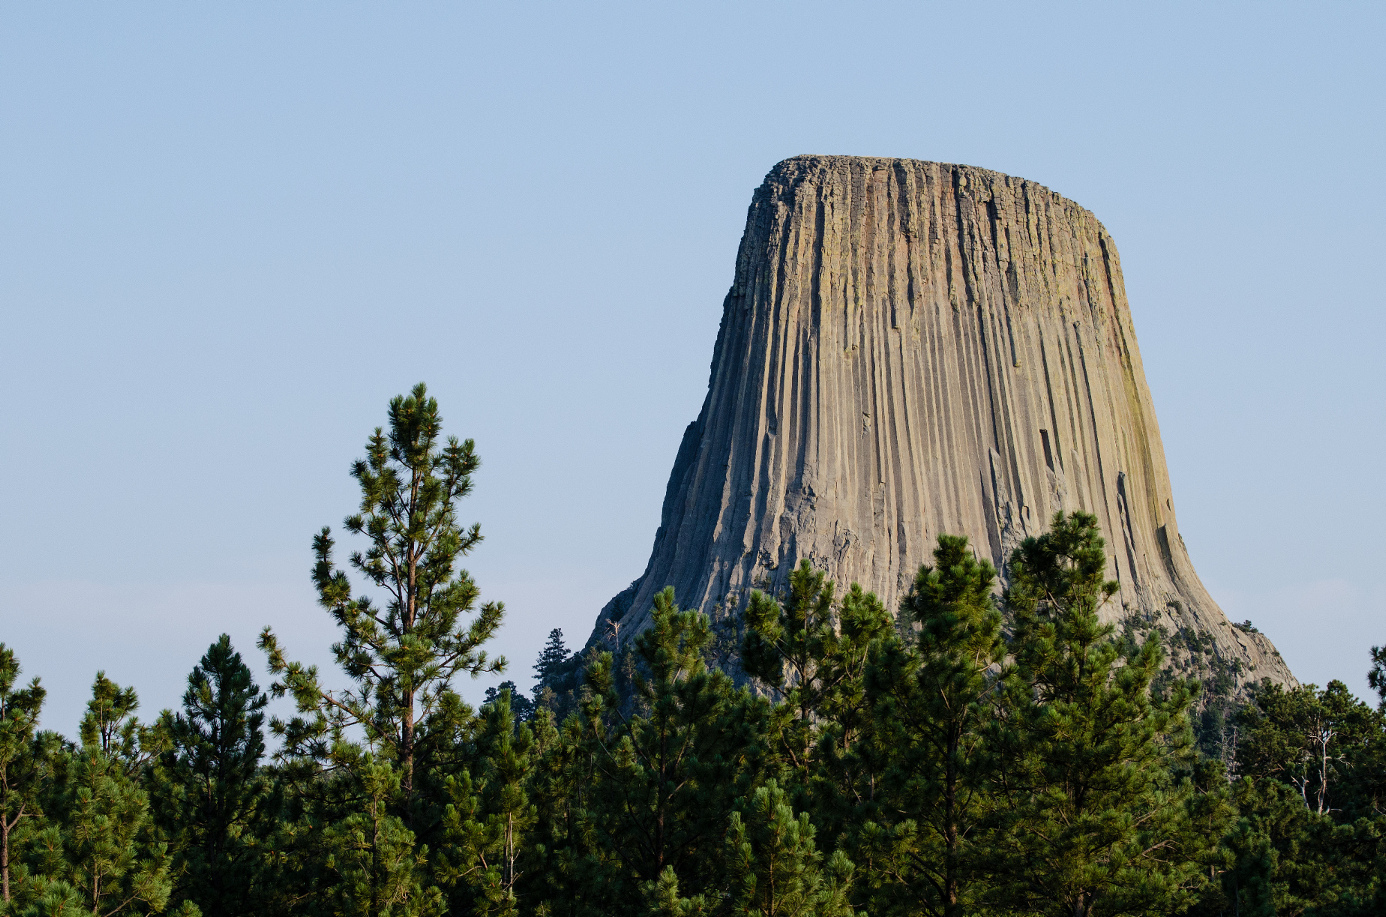
\includegraphics[width=0.75\textwidth]{devils_tower_bed_breakfast.jpg}}
\caption{I snapped this shot of the Devil's Tower from a nearby Bed and Breakfast. The skies
were bright blue and dull.} 
\label{fig:7048X1}
\end{figure}

To replace the dull sky in this shot I'd generate a mask based on sky
color and then tweak the boundary to avoid including tower and tree
parts. \emph{Tweaking masks and selections is a time-consuming pain.}
Luminar AI eliminates the drudgery, pushing a few buttons yields this jazzed up shot: see Figure~\ref{fig:7048X2} on page~\pageref{fig:7048X2}.

%\href{https://conceptcontrol.smugmug.com/Themes/Manipulations/Fake-Pixels/i-jft2zQ3/A}{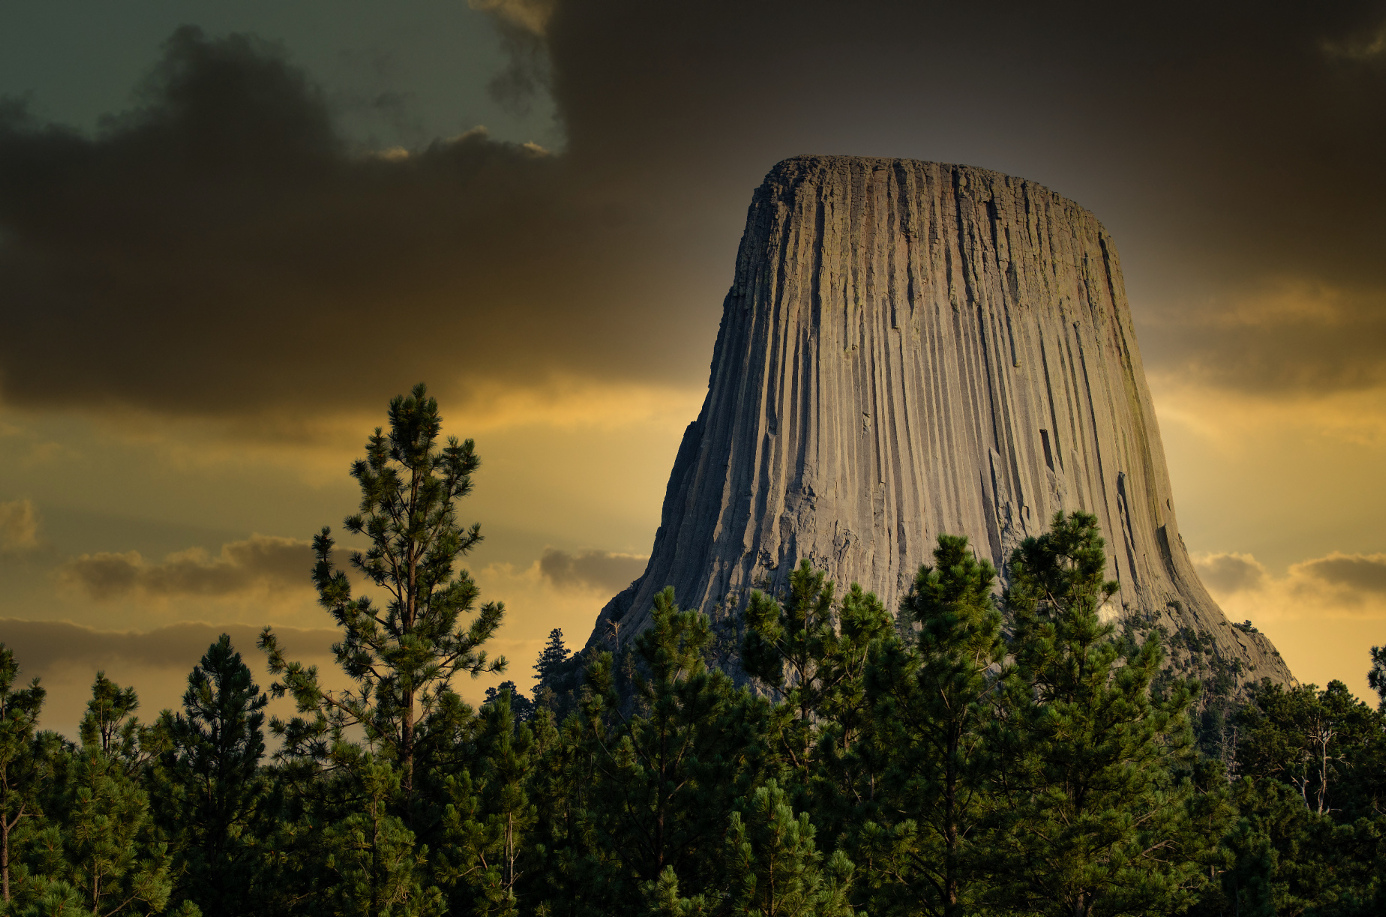
\includegraphics{devils_tower_fake_sky.jpg}}

%\captionsetup[figure]{labelformat=empty}
\begin{figure}[htbp]
\centering
\href{https://conceptcontrol.smugmug.com/Themes/Manipulations/Fake-Pixels/i-jft2zQ3/A}{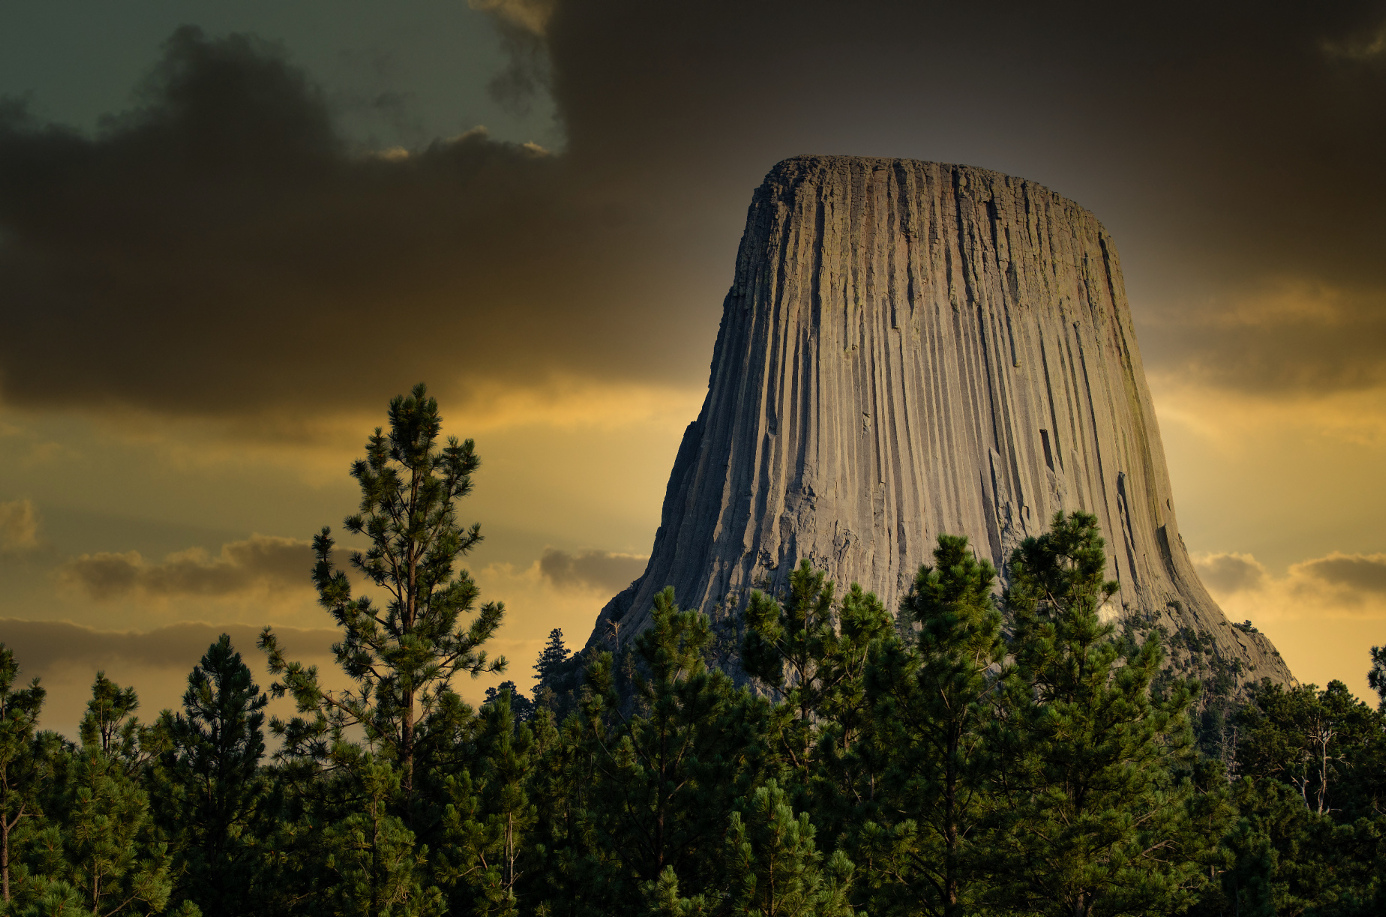
\includegraphics[width=0.75\textwidth]{devils_tower_fake_sky.jpg}}
\caption{\href{https://skylum.com/luminar-ai-b}{Luminar AI} makes short work of sky replacement. Now we
will have to restrain ourselves from over-applying this hack!} 
\label{fig:7048X2}
\end{figure}

Sky replacement has a long pedigree in photography. The practice started
with 19\textsuperscript{th}-century landscape photographers. They made
\emph{film} by mixing chemicals and spreading the mixture, called an
\emph{emulsion}, on large glass plates. Plate emulsions were very slow,
(would you believe an
\href{https://en.wikipedia.org/wiki/Film_speed}{effective ASA} below
four?), and
\href{https://www.nytimes.com/2012/10/12/arts/design/faking-it-at-the-met-a-photography-exhibition.html}{``disproportionately
sensitive to blue and violet light, resulting almost always in
overexposed skies.''} To fix their washed-out
skies\footnote{Hacking skies in paintings probably 
goes way back to cave and rock artists.
} 19\textsuperscript{th}-century photographers resorted to darkroom
trickery. Luminar AI has greatly streamlined this old image hack.

There's more to Luminar AI than sky replacement. I've found its portrait
and face manipulation features useful. The program does a very good job
of isolating eyes in images. Consider this diptych of a boy holding
dollars: Figure~\ref{fig:7048X3} on page~\pageref{fig:7048X3}

%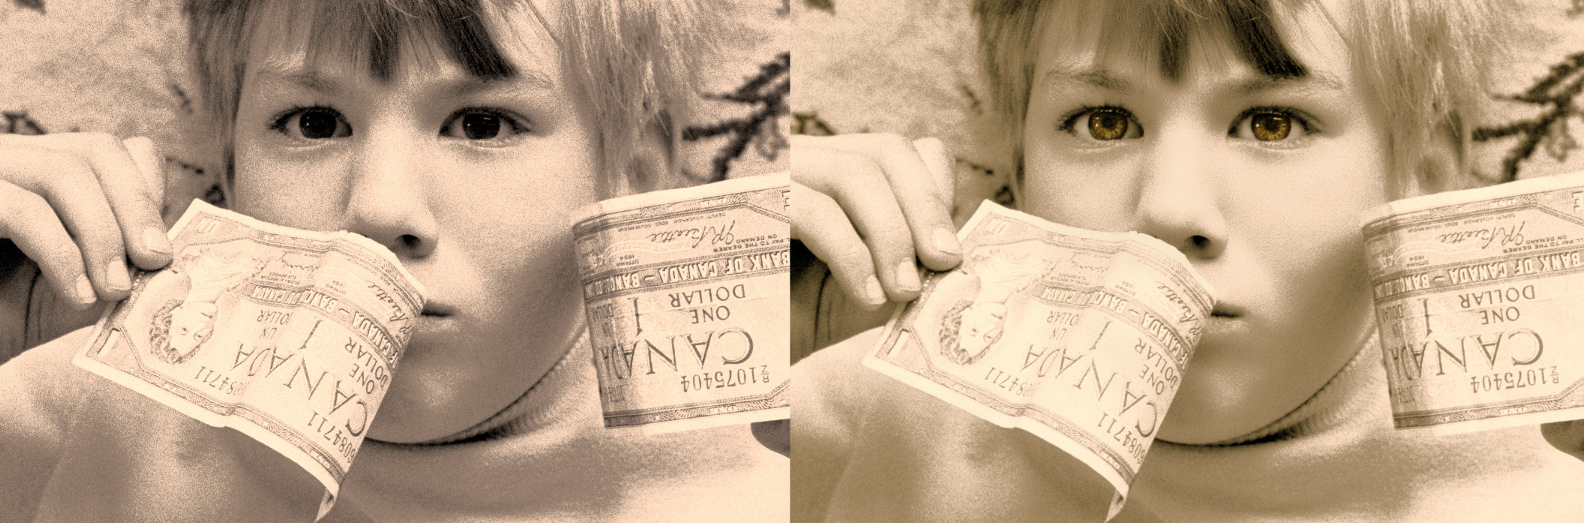
\includegraphics{eyes_before_after.jpg}

%\captionsetup[figure]{labelformat=empty}
\begin{figure}[htbp]
\centering
\href{https://bakerjd99.files.wordpress.com/2021/01/eyes_before_after.jpg}{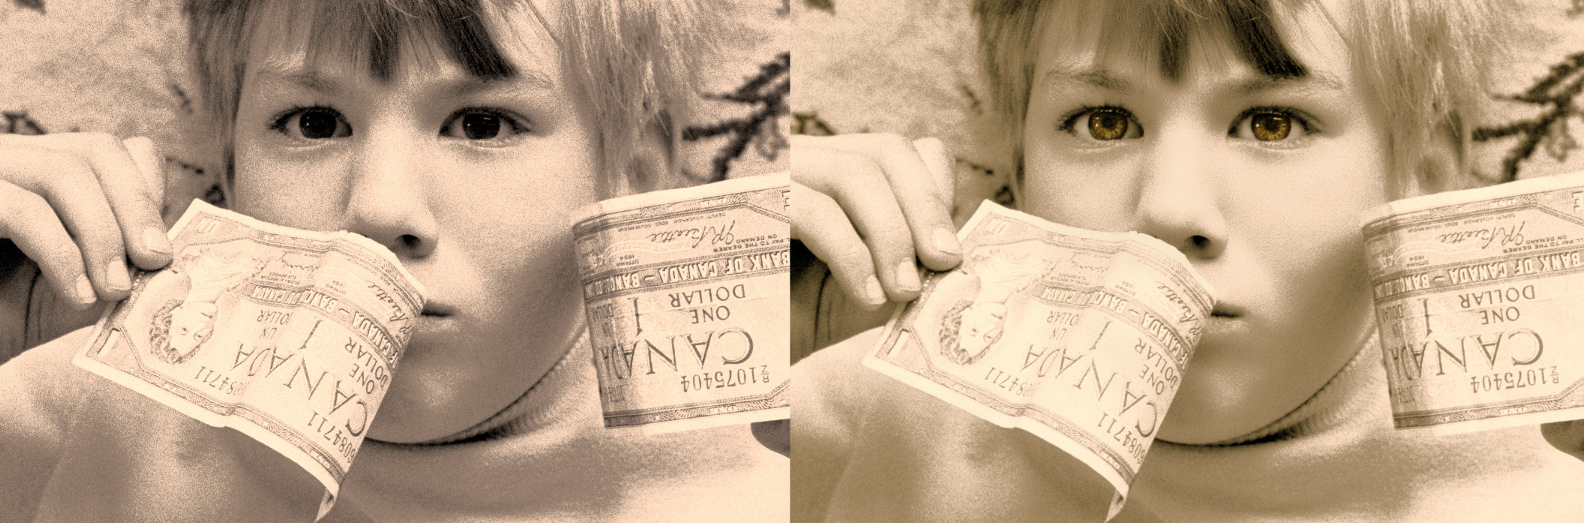
\includegraphics[width=0.75\textwidth]{eyes_before_after.jpg}}
\caption{Luminar AI easily isolates eyes and skin. Here I 
replaced the original's (left)  \emph{pit eyes} and softened skin.} 
\label{fig:7048X3}
\end{figure}

The original, on the left, has dark pit eyes. The Luminar AI version on
the right has enlarged fake eyes and model smooth skin. You wouldn't
normally push pixels this hard but sometimes a little eye and skin
tuning can make a portrait pop. I've only used Luminar AI for a few
weeks but it's already earned a spot on my image tools team.

\paragraph{Picture Window Pro 8}\label{picture-window-pro-8}

My next editor, \href{https://www.dl-c.com/Downloads.html}{Picture
Window Pro 8}, is a new version of what I have long considered the
``best bang for your buck'' image editor out there. I found Picture
Window Pro back in 2003. I was looking for an inexpensive editor that
could handle 16-bit channel images. Photoshop Elements, my second image
editor, only supported 8-bit images and full Photoshop was way too
expensive.\footnote{Some things never change, in 2021 Photoshop is still too expensive and
  now you are forced to \emph{subscribe} to
  it.} Adobe's larceny
drove me to Picture Window Pro (PWP) but once I there I never looked
back. PWP was much faster and more memory efficient than Photoshop and
it's many competitors. Traits that it maintains to this day. In 2021
it's still the fastest loading editor I use.

I stuck with Picture Window Pro from 2003 to 2017, longer than most
marriages. But, in 2017 Jonathan Sachs, the gifted developer of PWP,
decided to retire the program. It was PWP's retirement that led me to
start trying out new image editors every year. My first post PWP editor
was \href{https://affinity.serif.com/en-gb/photo/}{Affinity Photo}.
Affinity Photo is a fine tool that I use all the time,
\href{https://analyzethedatanotthedrivel.org/2017/01/22/affinity-photo-review/}{see
my review here}, but I missed PWP. So I was delighted when Picture
Window Pro 8 emerged.

Picture Window Pro 8 (PWP8) has revamped the older program for modern
large displays. You can now scatter PWP8 windows all over your giant
monitor. The program has also introduced a well considered
transformation history feature that makes it easy to track and reproduce
long edit chains.

%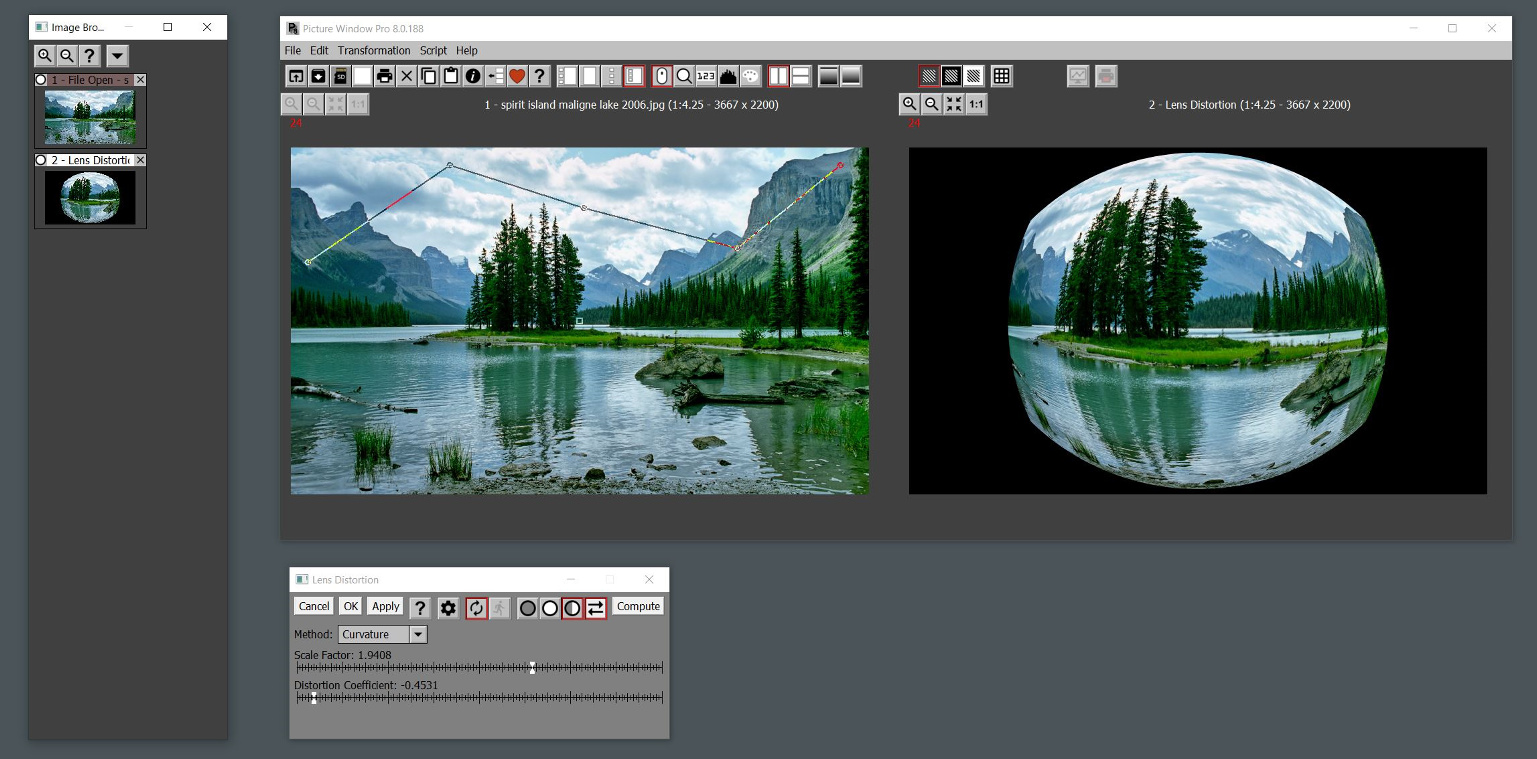
\includegraphics{pwp8screen.jpg}

\captionsetup[figure]{labelformat=empty}
%\begin{figure}[htbp]
%\centering
 \begin{SCfigure}[50]
 \centering
\href{https://bakerjd99.files.wordpress.com/2021/01/pwp8screen.jpg}{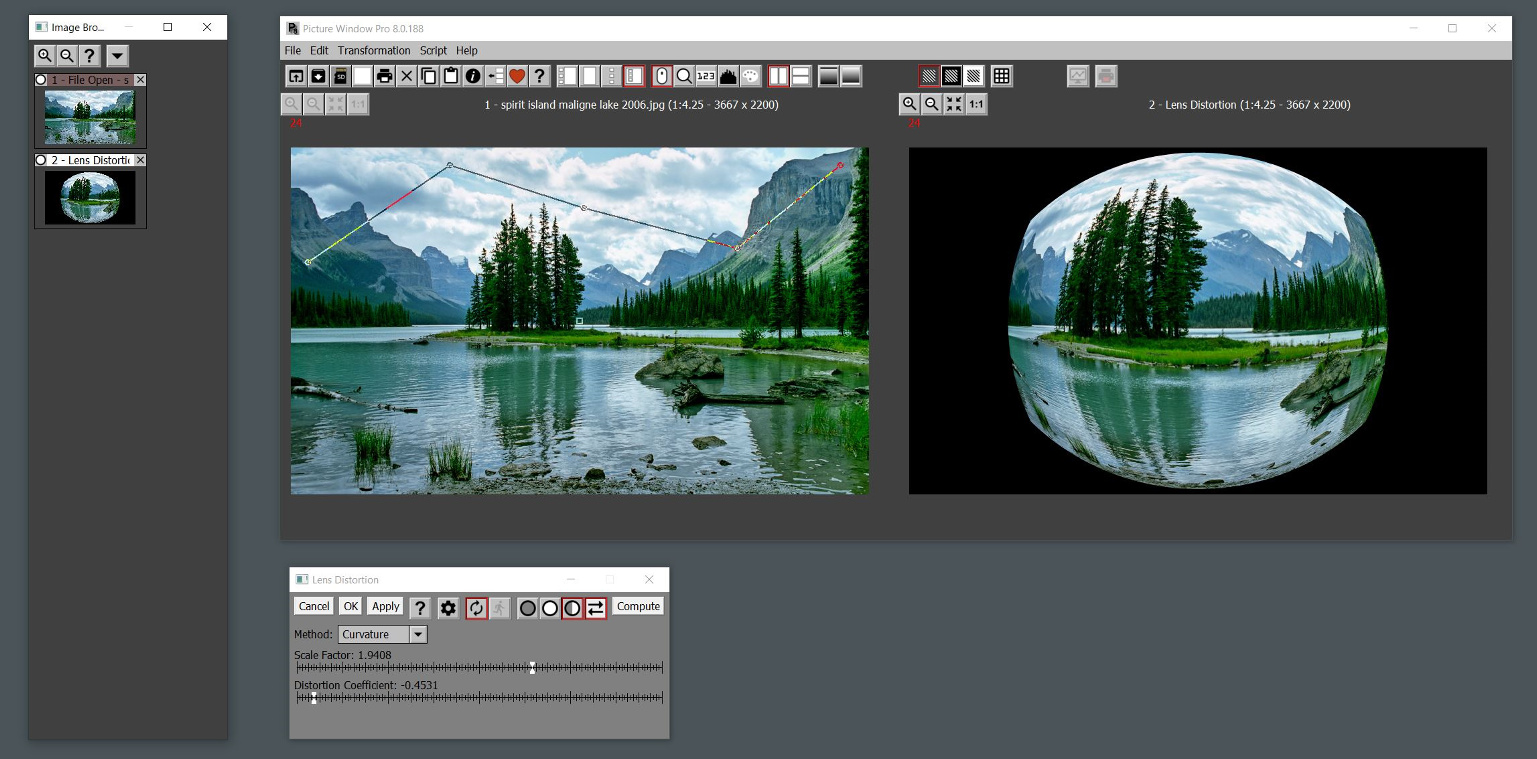
\includegraphics[width=0.65\textwidth]{pwp8screen.jpg}}
\caption{Unlike its predecessors \href{https://www.dl-c.com/Downloads.html}{Picture Window Pro 8} lets you to
spread  windows all over large screens.} 
\label{fig:7048X4}
\end{SCfigure}
%\end{figure}


And, if you thought PWP delivered bang for the buck, PWP8 takes it to a
new level. PWP8 is free for personal and commercial use. The developers
ask you to make a small PayPal donation: a fee I gladly paid. High
quality free is a killer combination! If you edit images on Windows
machines you owe it to yourself to get PWP8.

\paragraph{GNU GIMP 2.10.22}\label{gnu-gimp-2.10.22}

\href{https://www.gimp.org/}{GNU GIMP}, or ``The GIMP,'' as its
affectionately known, is a venerable open source system that's undergone
major upgrades in recent years. The most significant change has been the
edition of high bit channel support. The GIMP now supports 16-bit
channels and new high bit image formats like
\href{https://www.macworld.co.uk/feature/what-is-heic-3660408/}{HEIC}.
This puts the GIMP on par with commercial editors.

I've always liked the GIMP's vast potpourri of image hacking addins. You
can tell that few marketers and product designers were involved in their
development. Some guy, and let's be honest ladies it was probably a guy,
had an image edit itch and cranked out a GIMP addin to scratch it. This
explains the existence of, ``nobody asked for that,'' tools like mapping
images onto cubes and cylinders.

%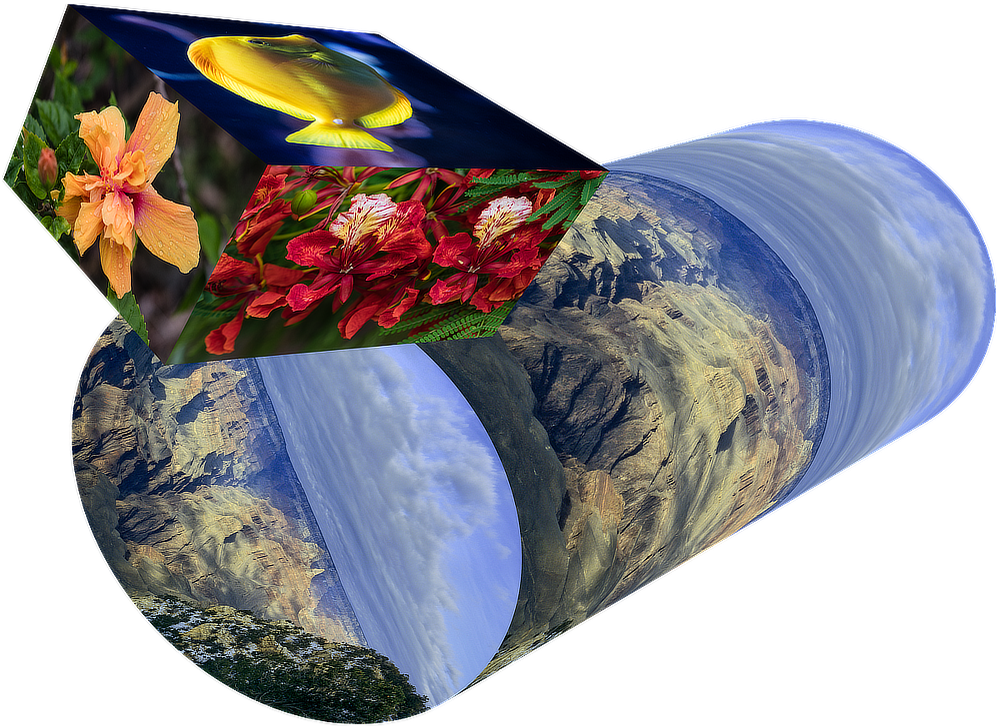
\includegraphics[width=5.20833in,height=3.79167in]{https://bakerjd99.files.wordpress.com/2021/01/fishcanyon.png}

%\captionsetup[figure]{labelformat=empty}
%\begin{figure}[htbp]
%\centering
%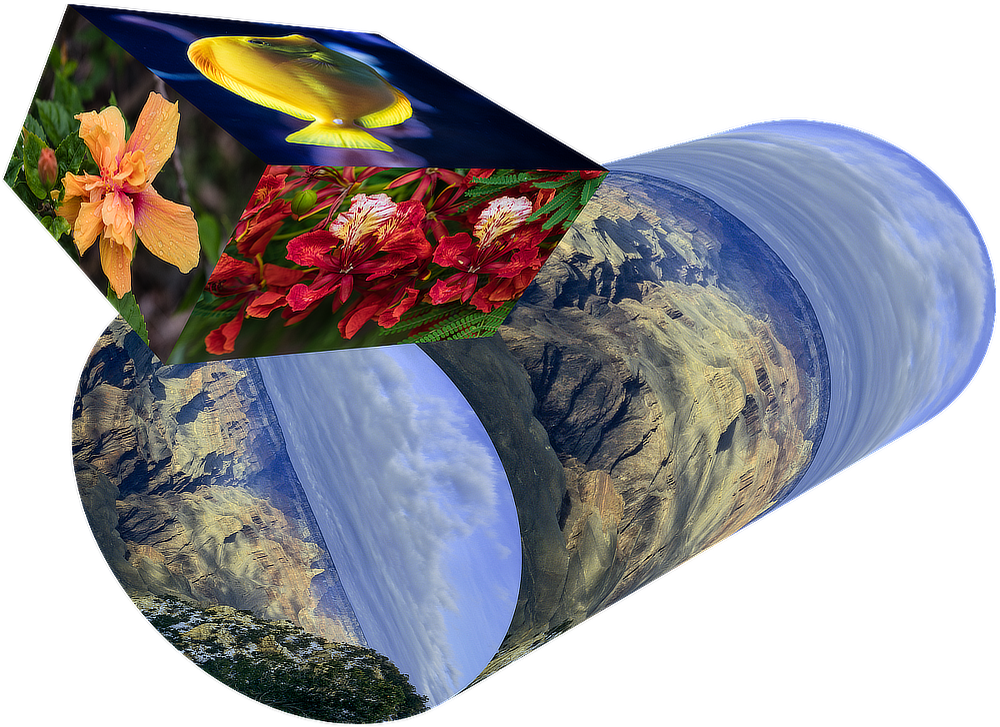
\includegraphics[width=0.40\textwidth]{cube_and_tube.png}
%\label{fig:7048X5}
%\end{figure}

% captions beside figure
\captionsetup[figure]{labelformat=empty}
\begin{SCfigure}
\centering
\href{https://conceptcontrol.smugmug.com/Themes/Manipulations/Alpha-Layered/i-HjsC9Lp/A}{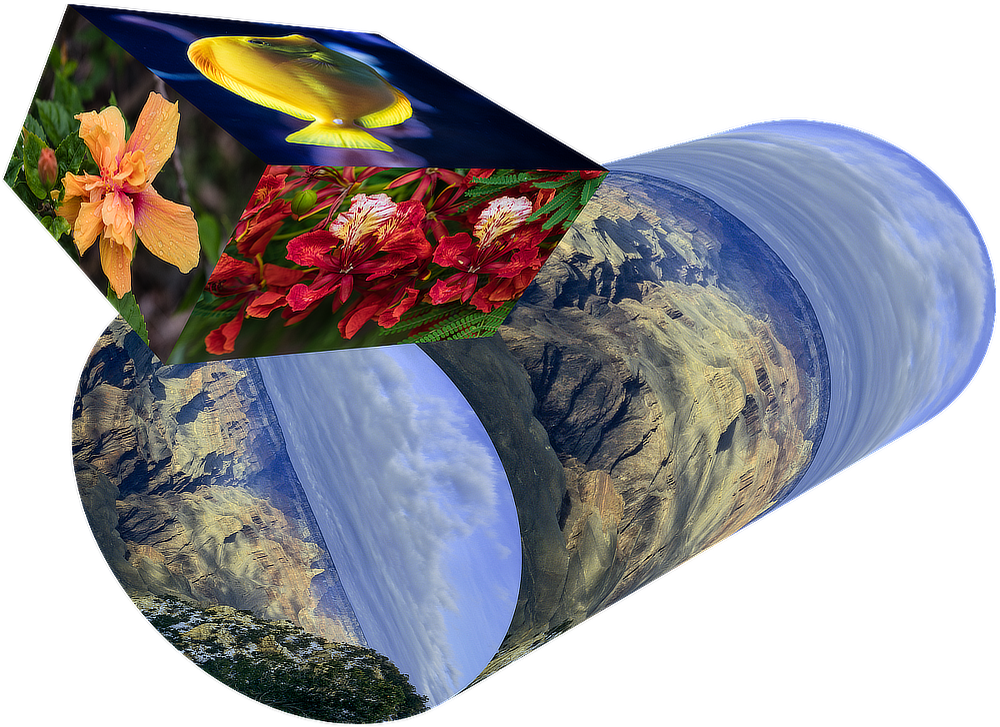
\includegraphics[width=0.40\textwidth]{cube_and_tube.png}}
\caption{\href{https://www.gimp.org/}{The GIMP} is loaded with odd addins that
you're unlikely to find in other image editors.}
\label{fig:7048X5}
\end{SCfigure}

The GIMP is fun, sprawling, capable, comprehensive, idiosyncratic, and
free: really free! If you're so inclined you can fetch
\href{https://gitlab.gnome.org/GNOME/gimp}{GIMP source code} and build
your own version. Sadly, this freedom has been abused. A fragile
\emph{wokester} that considered the word ``GIMP,'' which stands for
\textbf{G}NU \textbf{I}mage \textbf{M}anipulation \textbf{P}rogram,
\emph{ableist}\footnote{We can be thankful it still \emph{identifies} as a
  program!} has
\href{https://thenextweb.com/dd/2019/08/28/developer-forks-gimp-image-editor-over-naughty-name/}{forked
The GIMP and built a renamed version} that supposedly won't melt
effeminate snowflakes. \textbf{I am completely fed up with
\emph{wokespeak}; I will always call The GIMP ``The GIMP'' and so should
you!}

%\end{document}

%\begin{center}\rule{0.5\linewidth}{\linethickness}\end{center}

%\begin{enumerate}
%\item
%  \hypertarget{fn1}{}
%
%  New to me!\protect\hyperlink{fnref1}{↩︎}
%\item
%  \hypertarget{fn2}{}
%
%  Hacking skies in paintings probably goes way back to cave and rock
%  artists.\protect\hyperlink{fnref2}{↩︎}
%\item
%  \hypertarget{fn3}{}
%
%  Some things never change, in 2021 Photoshop is still too expensive and
%  now you are forced to \emph{subscribe} to
%  it.\protect\hyperlink{fnref3}{↩︎}
%\item
%  \hypertarget{fn4}{}
%
%  We can be thankful it still \emph{identifies} as a
%  program!\protect\hyperlink{fnref4}{↩︎}
%\end{enumerate}

 
% standard floating figure
% \captionsetup[figure]{labelformat=empty}
% \begin{figure}[htbp]
% \centering
% \href{}{\includegraphics[width=0.50\textwidth]{}}
% \caption{}
% \label{fig:????x0}
% \end{figure}
 
% captions beside figure
% \captionsetup[figure]{labelformat=empty}
% \begin{SCfigure}
% \centering
% \href{}{\includegraphics[width=0.40\textwidth]{}}
% \caption{}
% \label{fig:????x0}
% \end{SCfigure}

